% !TEX root = ../main.tex

\subsection{Simply support rectangular plate with sinusoidal transverse load}\label{sec:sinusoidal}

Considering a simply supported rectangular plate with domain $\Omega=(0,1)\otimes(0,1)$, whose material and geometric properties are $D=1$, Poisson's ratio $\nu=0.3$, and length $L=1$.
A sinusoidal transverse load of $\bar q = \sin(\pi x) \sin(\pi y)$ is subjected in $\Omega$, the corresponding analytical solution is stated as:
\begin{equation}\label{sinusoidal_w}
	w = 4\pi^{-4}\sin(\pi x) \sin(\pi y)
\end{equation}
The problem is sketched in Fig. \ref{fig:sinusoidal_plate}.

\begin{figure}[pos=htbp]
\centering
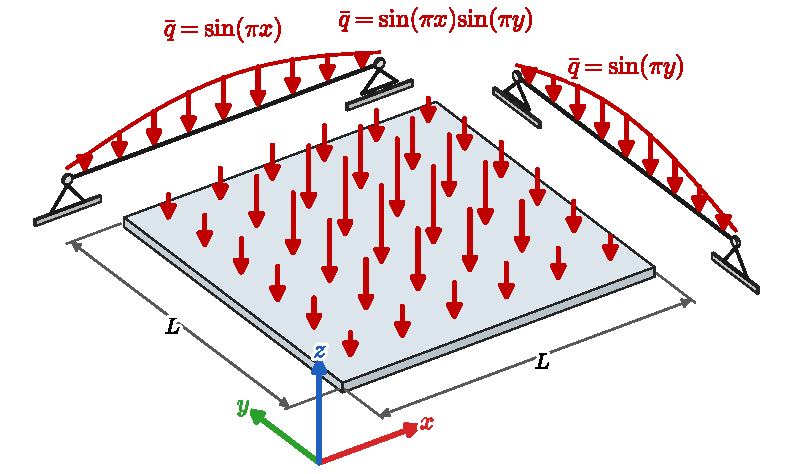
\includegraphics[width=\textwidth]{figs/sinusoidal_plate.pdf}
\caption{Simply supported square plate under the sinusoidal transverse load $\bar q=\sin(\pi x)\sin(\pi y)$: the two 1D models above the plate are its projections along $y$ (left) and along $x$ (right), drawn as calculation diagrams of a simply supported beam of the same length $L$, and the length of each load arrow on the plate follows $\bar q$ at its foot.}\label{fig:sinusoidal_plate}
\end{figure}
